\documentclass[letterpaper, 12pt]{article}

%% Language and font encodings
\usepackage[english]{babel}
\usepackage[utf8x]{inputenc}
\usepackage[T1]{fontenc}

%% Sets page size and margins
\usepackage[letterpaper,top=2.5cm,bottom=2cm,left=2cm,right=2cm,marginparwidth=1.75cm]{geometry}

%% Useful packages
\usepackage{amsmath}
\usepackage{amssymb}
\usepackage{amsfonts}
\usepackage{graphicx}
\usepackage{physics}
\usepackage{bbold}
\usepackage[colorinlistoftodos]{todonotes}
\usepackage[colorlinks=true, allcolors=blue]{hyperref}
\usepackage{listings}
\usepackage{multicol}
\usepackage{float}
\usepackage{enumitem}

\usepackage{bm}
\date{\today}

\title{CSC411 Assignment 3}
\author{Yue Guo}
\begin{document}
\maketitle

%%%%%%%%%%%Q1 	20 NEWS GROUP  %%%%%%%%%%%%%%
\section{20 News Group}
\subsection{Top 3 Algorithms}
Note: I have added a list of the names of all 20 categories in in load\_data( ) function for debugging purposes. This is does not affect my classification algorithm.

\subsubsection{Neural Network}
\begin{enumerate}

    \item Hypterparameter: number of layers
    
	Method: K-fold cross validation
	
	II have tried a single layer neural network vs multi-layered neural network.  It turns out that the single neural network is the fastest and also most accurate.

	\item Train/test loss
	\begin{itemize}
	
     \item  Train accuracy 0.974721583878
     \item Test accuracy 0.663303239511
        \end{itemize}
      
      \item Reason to pick this algorithm
      
      Neural network is commonly used in NLP, according to our lecture on neural networks. It is good at handling large data set with any features and produce a non-linear decision boundary.  
        
      \item My expectations
      
      This meets my expectation because NNs are good at working with a large dataset with many feartures. When I increase the number of hidden layers, accuracy decreases. I think this is because it overfits.
  
\end{enumerate}

\subsubsection{Random forest}
\begin{enumerate}

    \item Hypterparameter: number of estimators
    
	Method: K-fold cross validation

	I have tried Ensamble with 10 to 150 estimators, and 150 works best after comparing results from cross validation.

	\item Train/test loss
	\begin{itemize}
     \item  Train accuracy 0.974721583878
     \item Test accuracy 0.59346787042
        \end{itemize}
      
      \item Reason to pick Random forest
      I have tried decision tree, with different parameters(entropy vs gini) and reduced features, but all end up overfitting. Random forest introduces more randomness and also scales the weights of misclassified data in each iteration. To see decision tree, please uncomment from line 272 to 290 in q1.py.
      
      \item My expectations
      
      This meets my expectations because Random Forest adds more randomness in each step, and ensamble method is more resistant to overfitting because it assigns weights to different features in each step. I also tried decision\_tree, and it does not generalize well.
      The number of estimators learns better with a larger group of weak learners.
  
\end{enumerate}

\subsubsection{SVM - Best Classifier}
\begin{enumerate}

    \item Hypterparameter: rand\_state
    
	Method: K-fold cross validation

	In the code, I have tried different rand\_state and cross validated each. It turns out $rand\_state = 0$ is the best
	
	\item Train/test loss
	\begin{itemize}
     \item  Train accuracy  0.972511932119
     \item Test accuracy 0.691980881572
        \end{itemize}
        
 	\item Reason to pick SVM
	Because of the natural of this given problem, it is still a classification problem. Using neural nets might be an overkill. SVM produces a linear decision boundary with a margin for two classes. It can be extended to multi-class using algorithms such as one-vs-all.
        
          \item My expectations
     
      SVM is the best out of all. I think it is because it has a linear decision boundary with a margin and does not overfit on training data. The test accuracy is close to single neuron neural net, but still higher.
  

        
        \item Test confusion matrix
        
        The most confused classes are class 16 talk.politics.guns and 18 talk.politics.misc

\resizebox{\columnwidth}{!}{%
\setcounter{MaxMatrixCols}{20}
$\begin{matrix}
157.0 & 6.0 & 4.0 & 0.0 & 2.0 & 0.0 & 1.0 & 6.0 & 2.0 & 3.0 & 1.0 & 4.0 & 3.0 & 7.0 & 6.0 & 19.0 & 5.0 & 22.0 & 12.0 & 31.0 \\
2.0 & 278.0 & 19.0 & 12.0 & 3.0 & 47.0 & 3.0 & 1.0 & 3.0 & 2.0 & 2.0 & 7.0 & 9.0 & 9.0 & 10.0 & 2.0 & 2.0 & 1.0 & 1.0 & 4.0 \\
3.0 & 18.0 & 242.0 & 37.0 & 10.0 & 36.0 & 6.0 & 4.0 & 4.0 & 0.0 & 1.0 & 7.0 & 12.0 & 2.0 & 3.0 & 2.0 & 5.0 & 1.0 & 1.0 & 1.0 \\
2.0 & 8.0 & 37.0 & 254.0 & 35.0 & 9.0 & 14.0 & 3.0 & 1.0 & 4.0 & 0.0 & 3.0 & 26.0 & 1.0 & 2.0 & 1.0 & 2.0 & 4.0 & 2.0 & 2.0 \\
1.0 & 6.0 & 18.0 & 22.0 & 267.0 & 4.0 & 12.0 & 2.0 & 3.0 & 1.0 & 2.0 & 4.0 & 10.0 & 2.0 & 3.0 & 0.0 & 1.0 & 0.0 & 0.0 & 0.0 \\
0.0 & 24.0 & 14.0 & 9.0 & 4.0 & 273.0 & 0.0 & 2.0 & 0.0 & 1.0 & 0.0 & 4.0 & 8.0 & 1.0 & 2.0 & 1.0 & 0.0 & 0.0 & 0.0 & 1.0 \\
2.0 & 5.0 & 3.0 & 13.0 & 9.0 & 2.0 & 311.0 & 12.0 & 4.0 & 7.0 & 1.0 & 6.0 & 16.0 & 3.0 & 3.0 & 1.0 & 2.0 & 0.0 & 0.0 & 2.0 \\
7.0 & 3.0 & 3.0 & 2.0 & 6.0 & 0.0 & 6.0 & 282.0 & 21.0 & 3.0 & 3.0 & 3.0 & 9.0 & 6.0 & 8.0 & 2.0 & 7.0 & 1.0 & 6.0 & 3.0 \\
6.0 & 3.0 & 2.0 & 0.0 & 5.0 & 1.0 & 6.0 & 15.0 & 302.0 & 6.0 & 2.0 & 3.0 & 10.0 & 4.0 & 5.0 & 1.0 & 8.0 & 5.0 & 3.0 & 1.0 \\
12.0 & 10.0 & 18.0 & 8.0 & 14.0 & 6.0 & 11.0 & 28.0 & 16.0 & 329.0 & 23.0 & 19.0 & 14.0 & 15.0 & 18.0 & 15.0 & 13.0 & 12.0 & 9.0 & 9.0 \\
1.0 & 0.0 & 2.0 & 1.0 & 1.0 & 0.0 & 2.0 & 2.0 & 1.0 & 20.0 & 345.0 & 3.0 & 2.0 & 4.0 & 3.0 & 0.0 & 0.0 & 1.0 & 4.0 & 3.0 \\
2.0 & 6.0 & 2.0 & 2.0 & 4.0 & 3.0 & 1.0 & 1.0 & 0.0 & 1.0 & 2.0 & 282.0 & 12.0 & 1.0 & 1.0 & 0.0 & 8.0 & 4.0 & 3.0 & 2.0 \\
8.0 & 8.0 & 2.0 & 27.0 & 15.0 & 4.0 & 7.0 & 13.0 & 8.0 & 1.0 & 1.0 & 10.0 & 230.0 & 8.0 & 14.0 & 2.0 & 1.0 & 3.0 & 2.0 & 1.0 \\
8.0 & 0.0 & 4.0 & 0.0 & 0.0 & 2.0 & 0.0 & 3.0 & 7.0 & 4.0 & 3.0 & 2.0 & 12.0 & 302.0 & 7.0 & 7.0 & 6.0 & 2.0 & 5.0 & 7.0 \\
11.0 & 8.0 & 9.0 & 2.0 & 4.0 & 5.0 & 0.0 & 6.0 & 7.0 & 1.0 & 3.0 & 4.0 & 9.0 & 4.0 & 289.0 & 2.0 & 8.0 & 2.0 & 11.0 & 6.0 \\
44.0 & 1.0 & 1.0 & 0.0 & 2.0 & 1.0 & 2.0 & 1.0 & 5.0 & 6.0 & 2.0 & 4.0 & 2.0 & 7.0 & 5.0 & 319.0 & 11.0 & 11.0 & 3.0 & 63.0 \\
6.0 & 2.0 & 2.0 & 0.0 & 3.0 & 0.0 & 4.0 & 3.0 & 4.0 & 1.0 & 4.0 & 12.0 & 3.0 & 4.0 & 6.0 & 0.0 & 243.0 & 6.0 & 86.0 & 20.0 \\
13.0 & 2.0 & 3.0 & 0.0 & 0.0 & 0.0 & 1.0 & 5.0 & 2.0 & 0.0 & 1.0 & 3.0 & 2.0 & 6.0 & 2.0 & 1.0 & 9.0 & 283.0 & 7.0 & 6.0 \\
8.0 & 1.0 & 6.0 & 3.0 & 1.0 & 0.0 & 2.0 & 6.0 & 6.0 & 7.0 & 0.0 & 12.0 & 2.0 & 7.0 & 7.0 & 3.0 & 21.0 & 15.0 & 145.0 & 10.0 \\
26.0 & 0.0 & 3.0 & 0.0 & 0.0 & 2.0 & 1.0 & 1.0 & 2.0 & 0.0 & 3.0 & 4.0 & 2.0 & 3.0 & 0.0 & 20.0 & 12.0 & 3.0 & 10.0 & 79.0 \\
\end{matrix}%
$}



    \end{enumerate}

\subsubsection{Bernoulli Baseline}
\begin{enumerate}
	\item Train/test loss
	\begin{itemize}
     \item  Train accuracy  0.598727240587
     \item Test accuracy 0.457912904939
        \end{itemize}
\end{enumerate}





%%%%%%%%%%%Q2 SVM %%%%%%%%%%%%%%
\section{SVM}
\subsection{SVM test}
\begin{figure}[H]
\centering
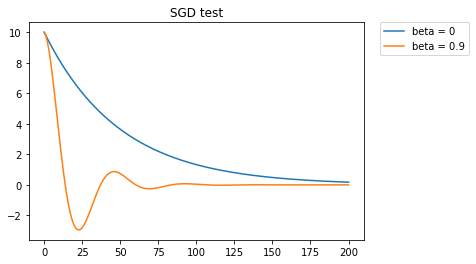
\includegraphics[width=0.5\textwidth]{q2part1plot.png}
\caption{\label{}Plot of test SVM}
\end{figure}

\subsection{SVM code}
see code

\subsection{SVM on MINIST}
\subsubsection{without momentum}
\begin{enumerate}
	\item Train loss$=0.400699029921$
	\item Test loss$=0.37243523202$
	\item classification accuracy on training set $= 0.826985854189$
	\item classification accuracy on testing set $=0.818503401361$
	\item Plot of w
	\begin{figure}[H]
\centering
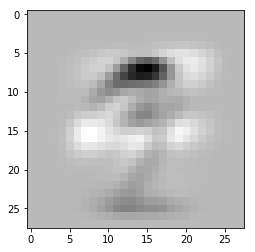
\includegraphics[width=0.5\textwidth]{q2_3_1.png}
\caption{\label{}Plot momentum = 0 }
\end{figure}
\end{enumerate}





\subsubsection{with momentum}
\begin{enumerate}
	\item Train loss = 0.424045274211
	\item Test loss = 0.394698671058
	\item classification accuracy on training set $= 0.817555313747$
	\item classification accuracy on testing set $=0.809977324263$
	\item Plot of w
	\begin{figure}[H]
	\centering
	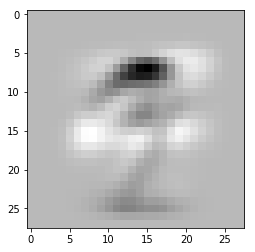
\includegraphics[width=0.5\textwidth]{q_2_3_2.png}
	\caption{\label{}Plot momentum = 0.1 }
	\end{figure}
\end{enumerate}





%%%%%%%%%%%Q3%%%%%%%%%%%%%%
\section{Kernels}
%%%%%%%%%% q 3.1%%%%%%%%%%%%%%
\subsection{Positive semidefinite and quadratic form}
Assume K is symmetric, we can decompose K into $U \Lambda U^T$
\begin{equation*}
\begin{split}
x^T K x &= x^T (U \Lambda U^T) x = (x^T U) \Lambda (U^T x)\\
\end{split}
\end{equation*}

$\Lambda$ has the eigenvalues $\lambda_{i}$, and if $K$ is positive, and all $\lambda_{i}$ > 0,

\begin{equation*}
\begin{split}
x^T K x &= \Sigma_{i =1}^{d} \lambda_{i} ([x^T U_{i}])^2 >= 0\\
\end{split}
\end{equation*}

Then $x^T K x >= 0$ for all $x$ in $ \mathbb{R}^{d}$ iff $K$ is postive semidefinite

%%%%%%%%%Q 3.2 %%%%%%%%%%%%%%
\subsection{Kernel properties}
%%%%%%%% Q 3.2 q2%%%%%%%%%%%%%
\subsubsection{$\alpha$}
Define mapping $\phi (x) = \sqrt{\alpha}$, $\alpha > 0$, and the kernel $\langle \phi(x), \phi(y) \rangle = \alpha$.
The resulting matrix K has item $K_{ij} = \alpha $, the matrix K has equal number of row and columns, and element is $\alpha$. Since $\alpha$ > 0, and all elements are equal, K is positive semidefinite
 
 %%%%%%%Q 3.2 q3 %%%%%%%%%%%%%%
\subsubsection{$f(x), f(y)$}
$K_{ij} = \langle \phi (x),  \phi (y) \rangle$, \\
define $\phi(x) = f(x), \forall f: \mathbb{R}^{d} \rightarrow \mathbb{R}$\\
define $\phi(y) = f(y), \forall f: \mathbb{R}^{d} \rightarrow \mathbb{R}$\\
Since f(x) and f(y) produce a scalar,  $\langle \phi (x),  \phi (y) \rangle = f(x) \cdot f(y)$

%%%%%%%%Q3.2 part 3%%%%%%%%%%%
\subsubsection{k1 and k2}
If the gram matrix, $K_{1}$ of kernel k1 and gram matrix, $K_{2}$ of kernel k2 are positive semidefinite, by scaling them and adding each element, the new gram matrix of $a \cdot k_{1}(x, y) + b \cdot k_{2}(x, y)$, call it $K$, each element of K is positive since a ,b > 0.\\
$K$ is also symmetric because $K_{1}$ and $K_{2}$ are symmetric with the same dimension, and element wise addition and linear combination preserve the symmetric property.\\

%%%%%%%%Q3.2 part 4%%%%%%%%%%%
\subsubsection{$k(x, y) = \frac{k_{1}(x ,y) }{\sqrt{k_{1}(x, x)} \sqrt{k_{1}(y, y)} }$}
Let $\phi_{1}$ be the mapping defined by $k_{1}$\\
We define a new mapping, $\phi$ for $k(x ,y)$\\
We let $\phi(x) = \frac{\phi_{1} (x)}{\norm{\phi_{1}(x)}}$\\
\begin{equation*}
\begin{split}
k(x, y) &= \langle \phi (x), \phi (y) \rangle \\
&= \frac{\phi_{1}(x)}{\norm{\phi_{1}(x)}} \cdot  \frac{\phi_{1}(y)}{\norm{\phi_{1}(y)}}\\
&= \frac{\phi_{1}(x)}{\sqrt{\phi_{1}(x) \cdot \phi_{1}(x)}} \cdot \frac{\phi_{1}(y)}{\sqrt{\phi_{1}(y) \cdot \phi_{1}(y)}}\\
&= \frac{\phi_{1}(x)}{( \sqrt{\phi_{1}(x)} \cdot \sqrt{ \phi_{1}(y)}  )}  \cdot \frac{\phi_{1}(y)}{( \sqrt{\phi_{1}(x)} \cdot \sqrt{ \phi_{1}(y)}  )} \\
&= \frac{\phi_{1}(x)}{ \sqrt{\phi_{1}(x) \cdot  \phi_{1}(y) }}  \cdot  \frac{\phi_{1}(x)}{ \sqrt{\phi_{1}(x) \cdot  \phi_{1}(y) }}\\
 k(x, y) &= \frac{k_{1}(x ,y) }{\sqrt{k_{1}(x, x)} \sqrt{k_{1}(y, y)} }
\end{split}
\end{equation*}
Therefore, there is a new mapping $\phi(x)$ that supports $k(x, y)$ and it is a kernel because $\phi(x)$
is the product of two kernel mappings

\end{document}